
%%SEE PRESENTATION FOLDER FOR SOURCE FILES%%%
\documentclass[english,t]{beamer}
% \documentclass[english,t,aspectratio=1610, 12pt,dvipsnames, table]{beamer}
\usepackage{beamer-JA}
\usepackage{tkz-euclide}
\DeclareMathAlphabet{\mathcal}{OMS}{cmsy}{m}{n}
\SetMathAlphabet{\mathcal}{bold}{OMS}{cmsy}{b}{n} %for big-O

%\beamerdefaultoverlayspecification{<+->}

%%%%Chapter and Section numbers%%%%% 
\newcommand{\chNum}{}
\newcommand{\secNum}{}
\newcommand{\secTitle}{Cauchy's Rigidity Theorem}
%\date{\formatdate{29}{9}{2015}}

%%%Title page%%%%%%%%
\title[Cool Math Meeting]{Cauchy's Rigidity Theorem}
% \day=21
% \month=8
% \year=2019 %remove to auo set date
\subtitle{}
\author{Jim Ashe}
%%change for windows/linux. note the forward slashes for windows!%%%
\titlegraphic{
\includegraphics[height=2.25cm]{pics_shared/WGU_logo.png}}
%%\titlegraphic{
\includegraphics[height=2.25cm]{/home/jim/Copy/schools/WGU/images/WGU_logo.png}}
\institute{IT College \\Computer Science}
%%%%%%%%%%%%%%%
\setbeamertemplate{caption}{\raggedright\insertcaption\par} %%removes label from figure captions
\tikzset{c/.style={every coordinate/.try,draw=#1!50!white}} %set for coord shift hack
\begin{document}
\makebeamertitle 
%%%%%%%%%%%%%%%
\begin{frame}{The back story} \label{slide-backstory}
The setting\dots
\begin{columns}
    \begin{column}{.6\textwidth}
        \begin{itemize}
            \item<2->It's the French revolution.
            \item<3->Legendre (\href{https://www.dictionary.com/browse/legendre}{l\textit{uh}-\textbf{zhahn}-\textit{druh}}) decides to translate the \textit{Elements}.
            \item<4->[] -all 13 books.
            \item<5->But he runs across a gap\dots
            \item<5->[] and hands it off to a 19 year old Cauchy. 
        \end{itemize}
    \end{column}
    \begin{column}{.4\textwidth}
        \only<2>{
        \begin{figure}
            \centering
            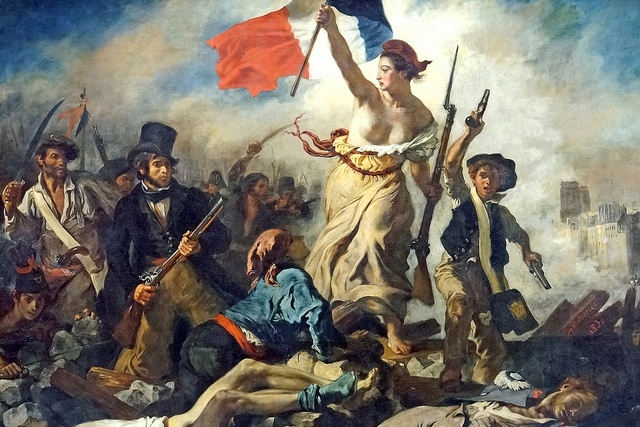
\includegraphics[width=\textwidth]{cauchy_images/Liberty-Leading-the-People.jpg}
            \caption{Viva la Revolution!}
            \label{fig:my_label}
        \end{figure}
        }
        \only<3-5>{
        \begin{figure}
            \centering
            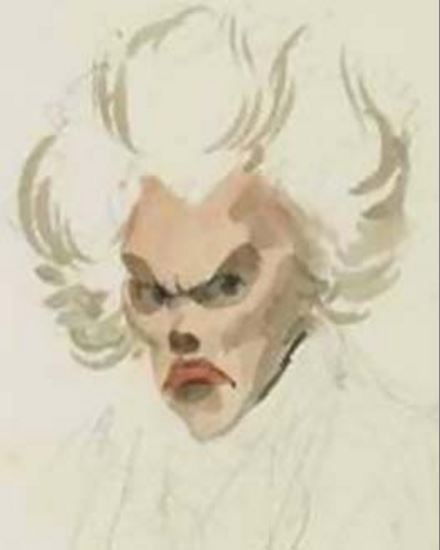
\includegraphics[width=.8\textwidth]{cauchy_images/Legendre.jpg}
            \caption{Legendre \footnotemark}
            \label{fig:my_label}
        \end{figure}
        }
        \only<6>{
        \begin{figure}
            \centering
            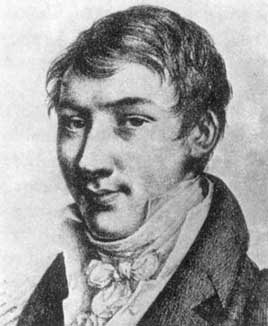
\includegraphics[width=\textwidth]{cauchy_images/Cauchy_2.jpeg}
            \caption{A young, hip Cauchy}
            \label{fig:my_label}
        \end{figure}
        }
    \end{column}
\end{columns}
    \only<3-5>{\footnotetext[1]{The only know picture of Legendre. For centuries there was a different picture shown in books. The mistake wasn't discovered until 2005.}}
\end{frame}

%%%new slide%%%%
\begin{frame}{Polyhedron problem} \label{old problem}
    \begin{figure}
        \centering
        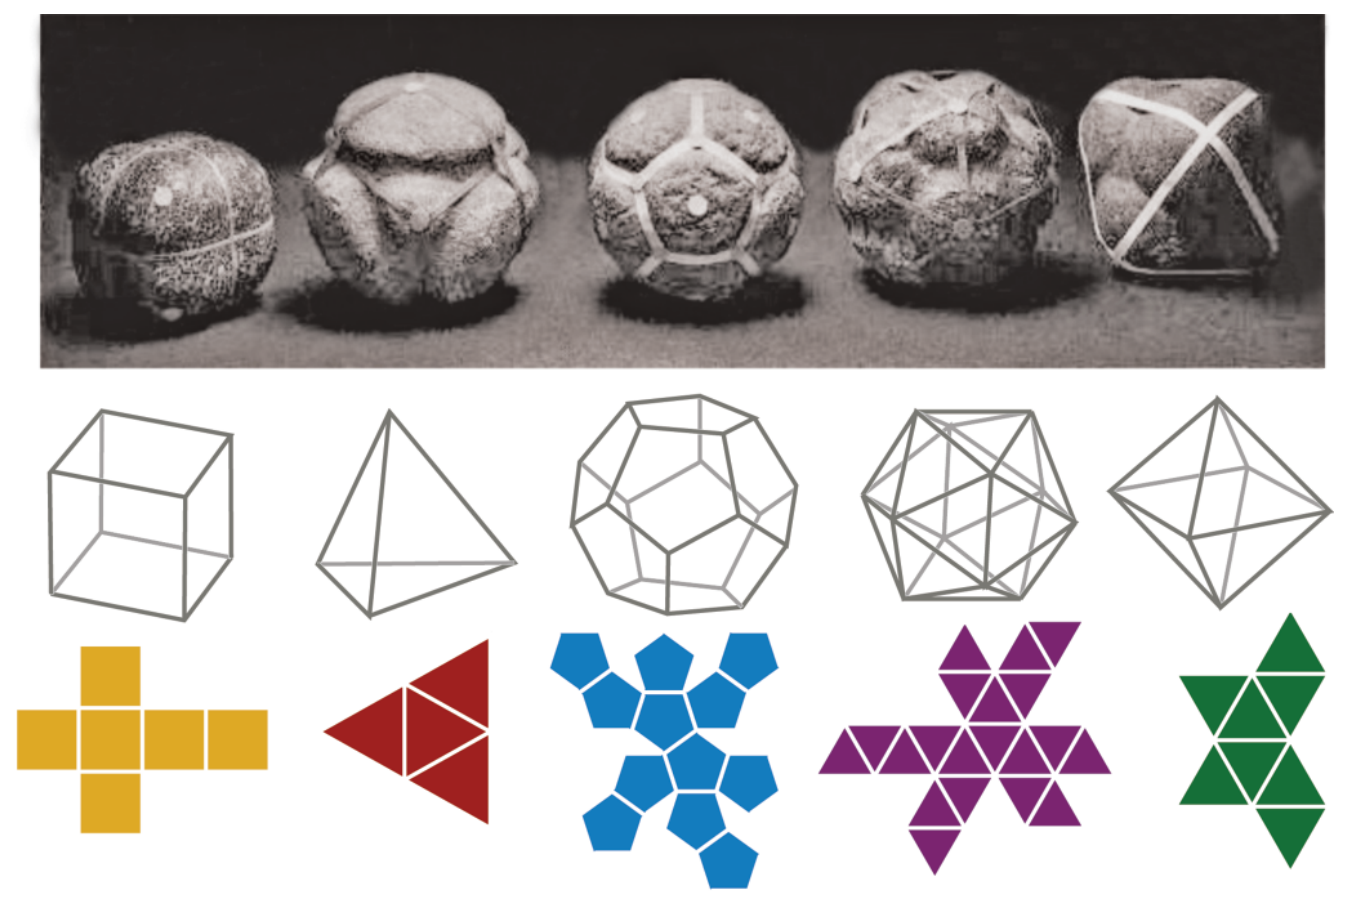
\includegraphics[width=\textwidth]{cauchy_images/2020-04-13_14h16_56.png}
        \caption{}
        \label{fig:my_label}
    \end{figure}
\end{frame}

%%%new slide%%%%
\begin{frame}{So what's the problem?}
    \only<1->{\textit{Equal and similar solid figures are those contained by similar planes equal in multitude and magnitude.}
    }\vspace{20pt}

    \only<2->{Let $P$ and $P\subset\mathbb{R}^{3}$ be two convex polytopes such that $\alpha(P)\simeq_{\pi}\alpha P'$, and for every 2-dimensional face $F$, $F\cong F^\prime$ (up to rigid motion by $O_{3}(\mathbb{R})\ltimes \mathbb{R}^{3}$, where $F'=\pi(F)$). Then $P\cong P^\prime$.
    }\vspace{20pt}
    
    \only<3->{\textit{Given the faces and gluing instructions, there is only one way to construct a polyhedron.}
    }
\end{frame}

%%%new slide%%%%
\begin{frame}{The problem\dots} \label{slide-1}
	\begin{columns}
	    \begin{column}{.6\textwidth}
    	    \only<1->{\begin{figure}
    	       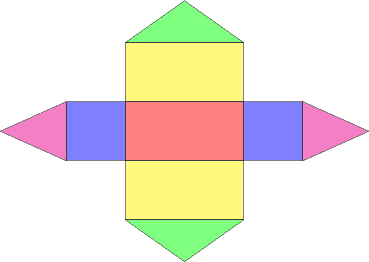
\includegraphics[width=\textwidth]{cauchy_images/unfolded_poly.pdf}
    	        \caption{Unfolded polyhedron}
    	        \label{fig:my_label}
    	    \end{figure}}
	    \end{column}
	    %%new column%%
	    \begin{column}{.4\textwidth}
	        \only<2>{
	        \begin{figure}
	            \vspace{25pt}
	            \centering     
	            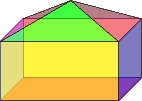
\includegraphics[width=\textwidth]{cauchy_images/convex_poly.pdf}
	            \caption{Convex polyhedron}
	            \label{fig:my_label}
	        \end{figure}
	        }
	        \only<3>{
	        \begin{figure}
	            \vspace{25pt}
	            \centering     
	            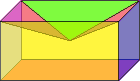
\includegraphics[width=\textwidth]{cauchy_images/nonconvex_poly.pdf}
	            \caption{Convexity matters!}
	            \label{fig:my_label}
	        \end{figure}
	        }
	        \vspace{.25in}
	    \end{column}
	\end{columns}
\end{frame}

%%%new slide%%%%
\begin{frame}{True for any convex polyhedron} \label{slide-2}
    \vspace{20pt}
    \begin{figure}
        \centering
        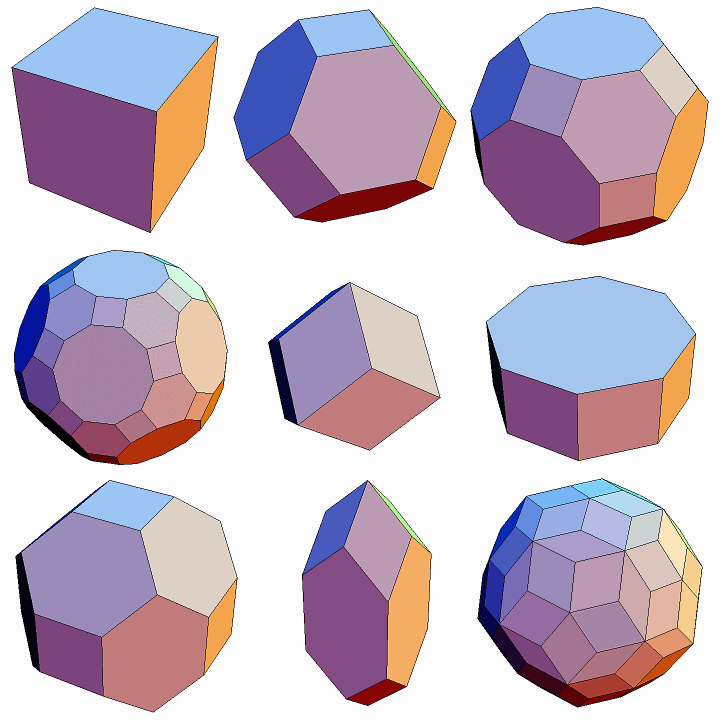
\includegraphics[width=.55\textwidth]{cauchy_images/poly_collection.png}
        \caption{}
        \label{fig:my_label}
    \end{figure}
\end{frame}

%%%new slide%%%%
\begin{frame}{So what can change?} \label{slide-3}
    \begin{columns}
        \begin{column}{.5\textwidth}
            \begin{itemize}
                \item<2-> Face angles fixed.
                \item<3-> Edge lengths fixed.
                \item<4-> "Gluing" instruction fixed.
                \item<5-> Only dihedral angles can change.
                \item[]<6-> "hinges"
            \end{itemize}
        \end{column}
        \begin{column}{.5\textwidth}
            \only<5-6>{
            \begin{figure}
                \centering
                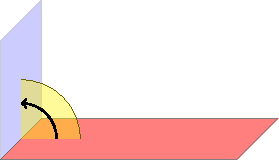
\includegraphics{cauchy_images/dihedral_90.pdf}
                \caption{}
                \label{fig:my_label}
            \end{figure}
            }
            \only<7>{
            \begin{figure}
                \centering
                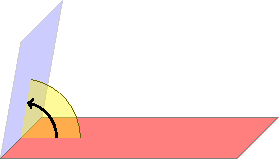
\includegraphics{cauchy_images/dihedral_80.pdf}
                \caption{}
                \label{fig:my_label}
            \end{figure}
            }
            \only<8>{
            \begin{figure}
                \centering
                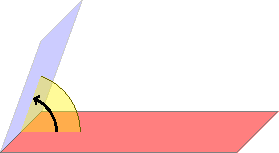
\includegraphics{cauchy_images/dihedral_70.pdf}
                \caption{}
                \label{fig:my_label}
            \end{figure}
            }
            \only<9>{
            \begin{figure}
                \centering
                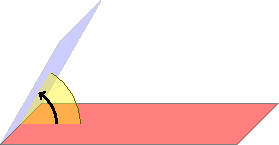
\includegraphics{cauchy_images/dihedral_60.pdf}
                \caption{}
                \label{fig:my_label}
            \end{figure}
            }
        \end{column}
    \end{columns}
\end{frame}

%%%new slide%%%%
\begin{frame}{Plan of attack} \label{plan of attack}
    \centering If it could change, what would happen?
    \begin{columns}
        \begin{column}{.5\textwidth}
            \begin{itemize}
                \item<2->What happens \textit{globally}? 
            \end{itemize}
            \only<2->{
            \begin{figure}
                \centering
                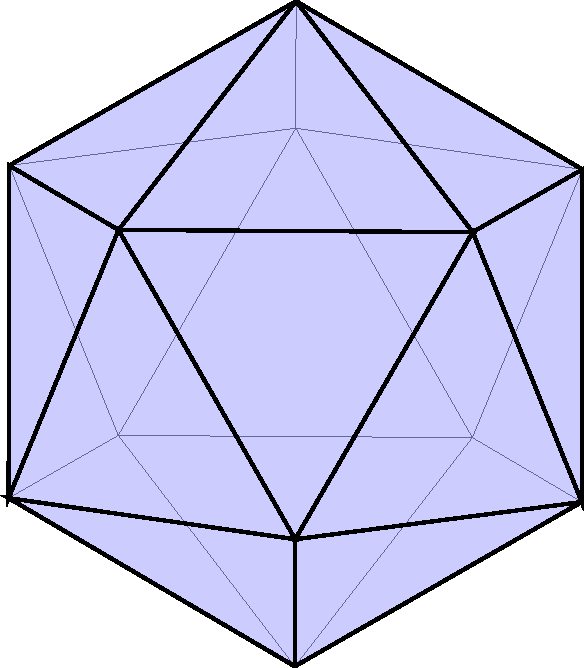
\includegraphics[width=.6\textwidth]{cauchy_images/deltahedron.pdf}%%deltahedron
                % \caption{}
                \label{fig:my_label}
            \end{figure}
            }%
            \only<4->{Global behavior $\Rightarrow$ upper limit on hinge angle changes.}
        \end{column}    
        \begin{column}{.5\textwidth}
            \begin{itemize}
                \item<3->What happens \textit{locally}?
            \end{itemize}
            \only<3->{
            \vspace{25pt}
            \begin{figure}
                \centering
                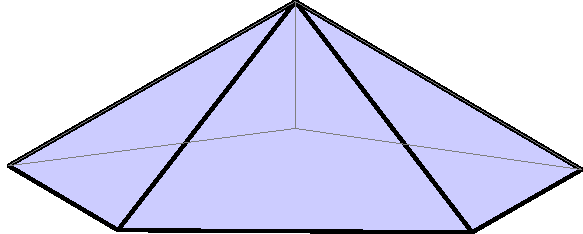
\includegraphics[width=.6\textwidth]{cauchy_images/deltahedron_top.pdf}%%deltahedron top
                % \caption{}
                \label{fig:my_label}
            \end{figure}
            }%
            \only<5->{Local behavior $\Rightarrow$ lower limit on hinge angles change.}
        \end{column}    
    \end{columns}
\end{frame}

%%%new slide%%%%
\begin{frame}{Local}\label{intersection with sphere}
    \only<1>{
    \vspace{25pt}
    \begin{figure}
        \centering
        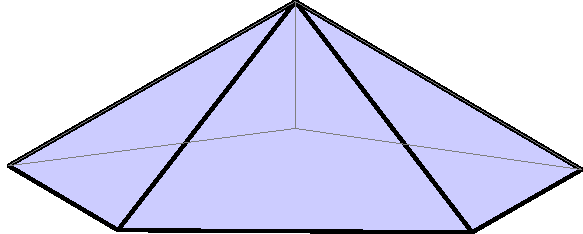
\includegraphics[width=.6\textwidth]{cauchy_images/deltahedron_top.pdf} %%delta -top
        \caption{vertex}
        \label{fig:my_label}
    \end{figure}
    }
    \only<2>{
    \begin{figure}
        \centering
        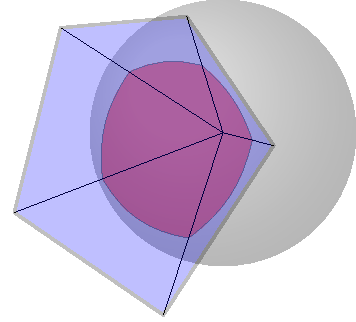
\includegraphics[width=.6\textwidth]{cauchy_images/sphere_and_cone.pdf} %%cone in sphere
        \caption{Stick the vertex into a sphere.}
        \label{fig:my_label}
    \end{figure}
    }
    \only<3>{
    \begin{figure}
        \centering
        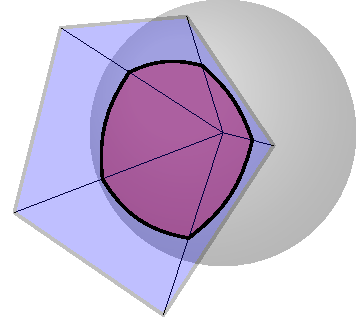
\includegraphics[width=.6\textwidth]{cauchy_images/sphere_and_cone_int.pdf} %%cone in sphere
        \caption{arcs = face angles}
        \label{fig:my_label}
    \end{figure}
    }
    \only<4>{
    \begin{figure}
        \centering
        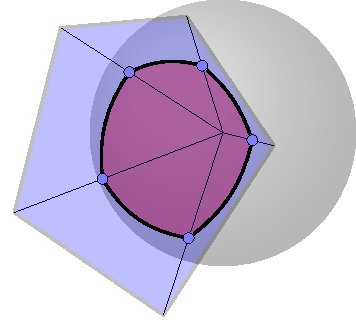
\includegraphics[width=.6\textwidth]{cauchy_images/sphere_and_cone_int_pts.pdf} %%cone in sphere
        \caption{intersection is a polygon}
        \label{fig:my_label}
    \end{figure}
    }
\end{frame}

%%%new slide%%%%
\begin{frame}{Polygon angles = hinge angles} \label{polygon angles = hinge}
    \only<1>{
    \begin{figure}
        \centering
        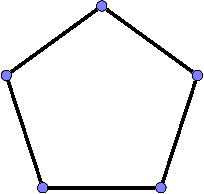
\includegraphics[width=.45\textwidth]{cauchy_images/poly-pentagon.pdf} %%polgon regular
        \caption{Polygon angles = hinge angles}
        \label{fig:my_label}
    \end{figure}
    }
    \only<2>{
    \begin{figure}
        \centering
        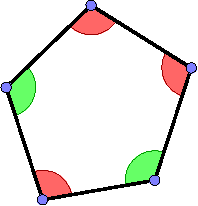
\includegraphics[width=.45\textwidth]{cauchy_images/poly-pentagon-squish0.pdf} %%polygon flex
        \caption{squishy}
        \label{fig:my_label}
    \end{figure}
    }
    \only<3>{
    \begin{figure}
        \centering
        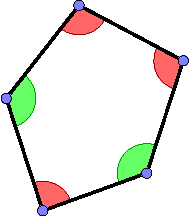
\includegraphics[width=.45\textwidth]{cauchy_images/poly-pentagon-squish1.pdf} %%polygon flex 2
        \caption{squishy}
        \label{fig:my_label}
    \end{figure}
    }
    \only<4>{
    \begin{figure}
        \centering
        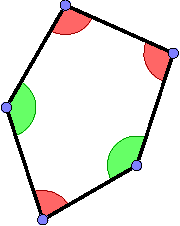
\includegraphics[width=.45\textwidth]{cauchy_images/poly-pentagon-squish2.pdf} %%polygon flex show angle changes
        \caption{squishier}
        \label{fig:my_label}
    \end{figure}
    }
    \only<5>{
    \begin{figure}
        \centering
        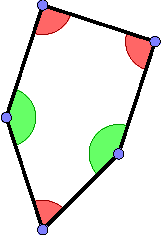
\includegraphics[width=.45\textwidth]{cauchy_images/poly-pentagon-squish3.pdf} %%polygon flex show angle changes
        \caption{squishiest}
        \label{fig:my_label}
    \end{figure}
    }
    \only<6>{
    Count the \textit{number} of changes. What's the least you can have? 
    \begin{figure}
        \centering
        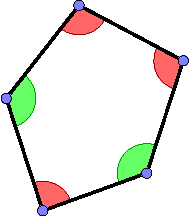
\includegraphics[width=.45\textwidth]{cauchy_images/poly-pentagon-squish1.pdf} %%polygon flex show angle changes
        \caption{Here we have 4 changes.}
        \label{fig:my_label}
    \end{figure}
    }
    \only<7>{
    What if we only have 2 changes? 
    \begin{figure}
        \centering
        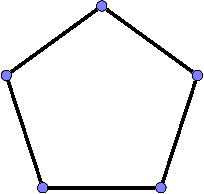
\includegraphics[width=.45\textwidth]{cauchy_images/poly-pentagon.pdf} %%polygon flex just 2 unbroken
        \caption{}
        \label{fig:my_label}
    \end{figure}
    }
    \only<8>{
    Cauchy's arm lemma: There must be at least 4 changes.
    \begin{figure}
        \centering
        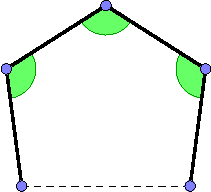
\includegraphics[width=.45\textwidth]{cauchy_images/arm_lemma_break.pdf} %%polygon flex just 2 BROKEN
        \caption{snap!}
        \label{fig:my_label}
    \end{figure}
    }
\end{frame}

%%%new slide%%%%
\begin{frame}{Cauchy's arm lemma} \label{arm lemma}
    \begin{columns}
        \begin{column}{.45\textwidth}
            \only<-7>{
            \begin{itemize}
                \item<2-> Law of cosines $\Rightarrow n=3$ case.
                \item<3-> Increase previous angles except $v_{2}$
                \item<4-> Increase $v_{2}$; reapply LOC. 
                \item<5-> Increase previous angles except $v_{3}$
                \item<6-> Increase $v_{3}$; reapply LOC. 
                \item<6-> $\dots$
            \end{itemize}
            }
            \only<8->{
            \begin{itemize}
                \item<8-> Law of cosines $\Rightarrow n=3$ case.
                \item<9-> If it's true for $n$
                \item<10-> then increase previous angles except $v_{n+1}$
                \item<11-> Reapply law of cosines.
                \item<12-> $\dots$
            \end{itemize}
            }
        \end{column}
        
        \begin{column}{.55\textwidth}
        \only<1>{
            \begin{figure}
                \centering
                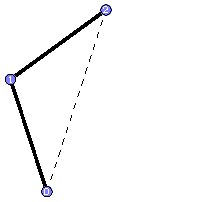
\includegraphics{cauchy_images/arm_lemma_induct_0-a.pdf}%%n=3
                \caption{$n=3$}
                \label{fig:my_label}
            \end{figure}
        }
        \only<2>{
            \begin{figure}
                \centering
                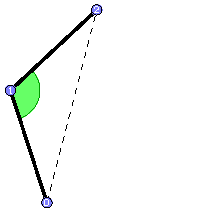
\includegraphics{cauchy_images/arm_lemma_induct_0-b.pdf}%%n=3
                \caption{$n=3$}
                \label{fig:my_label}
            \end{figure}
        }
        \only<3>{
            \begin{figure}
                \centering
                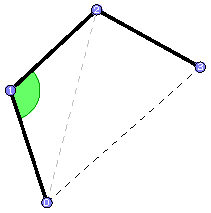
\includegraphics{cauchy_images/arm_lemma_induct_1-a.pdf}%%n=4
                \caption{$n=4$}
                \label{fig:my_label}
            \end{figure}
        }
        
        \only<4>{
            \begin{figure}
                \centering
                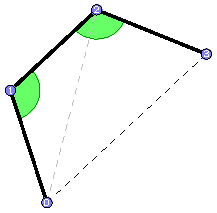
\includegraphics{cauchy_images/arm_lemma_induct_1-b.pdf}%%n=5
                \caption{$n=4$}
                \label{fig:my_label}
            \end{figure}
        }
        \only<5>{
            \begin{figure}
                \centering
                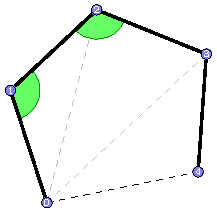
\includegraphics{cauchy_images/arm_lemma_induct_2-a.pdf}%%n=N
                \caption{$n=5$}
                \label{fig:my_label}
            \end{figure}
        }
        \only<6>{
            \begin{figure}
                \centering
                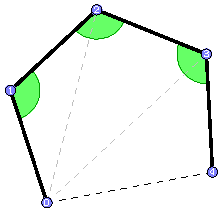
\includegraphics{cauchy_images/arm_lemma_induct_2-b.pdf}%%n=N
                \caption{$n=5$}
                \label{fig:my_label}
            \end{figure}
        }
        \only<7->{
            \begin{figure}
                \centering
                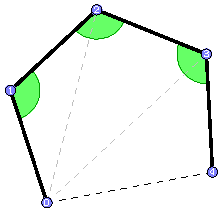
\includegraphics{cauchy_images/arm_lemma_induct_2-b.pdf}%%n=N
                \caption{$n=1,2,\dots$}
                \label{fig:my_label}
            \end{figure}
        }
        \end{column}
    \end{columns}
\end{frame}

%%%new slide%%%%
\begin{frame}{Cauchy's arm lemma \frownie} \label{arm lemma wrong}
    \begin{columns}
        \begin{column}{.4\textwidth}
            \only<1->{
            \vspace{25pt}
            \begin{itemize}
                \item<2-> Too bad this is wrong!
                \item<3-> the tragic loss of convexity.
                \item<4-> Unnoticed for +100 years. 
                \item<5-> Geometry is tricky!
            \end{itemize}
            }
        \end{column}
        
        \begin{column}{.6\textwidth}
        \vspace{30pt}
        \only<2>{
            \begin{figure}
                \centering
                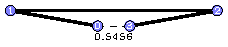
\includegraphics[width=.6\textwidth]{cauchy_images/convex_loss-0.pdf}%extreme shape%
                % \caption{$n=3$}
                \label{fig:my_label}
            \end{figure}
        }
        \only<3>{
            \begin{figure}
                \centering
                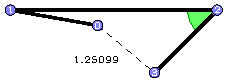
\includegraphics[width=.6\textwidth]{cauchy_images/convex_loss-1.pdf}%%loss of convexity
                \caption{Oops!}
                \label{fig:my_label}
            \end{figure}
        }
        \only<4->{
            \begin{figure}
                \centering
                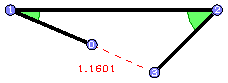
\includegraphics[width=.6\textwidth]{cauchy_images/convex_loss-2.pdf}%%n=5
                \caption{Everybody makes mistakes. Even geniuses.}
                \label{fig:my_label}
            \end{figure}
        }
        \end{column}
    \end{columns}
\end{frame}

%%%new slide%%%%
\begin{frame}{Cauchy's arm lemma \smiley} \label{arm lemma wrong 1}
    \begin{columns}
        \begin{column}{.45\textwidth}
            \only<1->{
            \vspace{25pt}
            \begin{itemize}
                \item<1-> Fortunately, there is a slick fix.
            \end{itemize}
            }
        \end{column}
        
        \begin{column}{.75\textwidth}
        \vspace{30pt}
        \only<1>{
            \begin{figure}
                \centering
                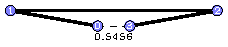
\includegraphics[width=.6\textwidth]{cauchy_images/convex_loss-0.pdf}%extreme shape%
                % \caption{$n=3$}
                \label{fig:my_label}
            \end{figure}
        }
        \only<2>{
            \begin{figure}
                \centering
                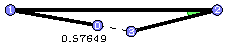
\includegraphics[width=.6\textwidth]{cauchy_images/convex_fix-0.pdf}%%loss of convexity
                \label{fig:my_label}
            \end{figure}
        }
        
        \only<3>{
            \begin{figure}
                \centering
                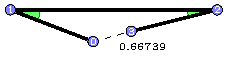
\includegraphics[width=.6\textwidth]{cauchy_images/convex_fix-1.pdf}%%n=5
                \label{fig:my_label}
            \end{figure}
        }
        
        \only<4>{
            \begin{figure}
                \centering
                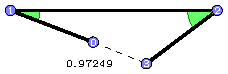
\includegraphics[width=.6\textwidth]{cauchy_images/convex_fix-2.pdf}%%n=5
                \label{fig:my_label}
            \end{figure}
        }
        
        \only<5>{
            \begin{figure}
                \centering
                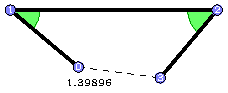
\includegraphics[width=.6\textwidth]{cauchy_images/convex_fix-3.pdf}%%n=5
                \label{fig:my_label}
            \end{figure}
        }
        \end{column}
    \end{columns}
    \vspace{25pt}
    \only<6->{
        \textbf{Cauchy's arm lemma $\Rightarrow$} a \textit{local} condition:\\
        \textit{The number of changes (from $+$  to $-$) at a vertex is $\geq$ 4.}
    }
\end{frame}

%%%new slide%%%%
\begin{frame}{Global} \label{arm lemma wrong 2}
    \begin{columns}
        \begin{column}{.45\textwidth}
            \only<1->{
            \vspace{25pt}
            \begin{itemize}
                \item[]<6->The geometry is gone.
                \item<7->vertices = $V = \only<7->{5}$ 
                \item<8->edges = $E = \only<8->{8}$ 
                \item<9->faces = $F = \only<9->{5}$
                \item<10-> $5-8+5=2$ 
            \end{itemize}
            }
        \end{column}
        
        \begin{column}{.6\textwidth}
        \only<1>{
            \begin{figure}
                \centering
                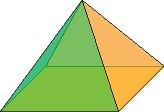
\includegraphics[width=.6\textwidth]{cauchy_images/pyramid.pdf}%extreme shape%
                \caption{any polyhedron}
                \label{fig:my_label}
            \end{figure}
        }
        \vspace{-10pt}
        \only<2>{
            \begin{figure}
                \centering
                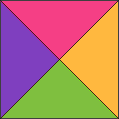
\includegraphics[width=.6\textwidth]{cauchy_images/pyramid-euler-0.pdf}%%loss of convexity
                \caption{can be flattened out}
                \label{fig:my_label}
            \end{figure}
        }
        \only<3>{
            \begin{figure}
                \centering
                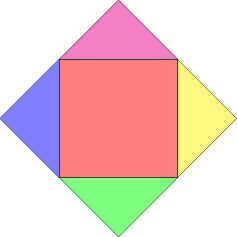
\includegraphics[width=.6\textwidth]{cauchy_images/pyramid_unfolded.pdf}%%loss of convexity
                \caption{can be flattened out}
                \label{fig:my_label}
            \end{figure}
        }
        \only<4>{
            \begin{figure}
                \centering
                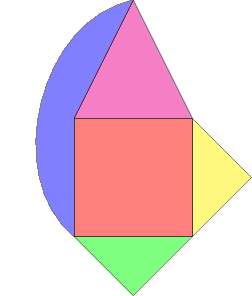
\includegraphics[width=.6\textwidth]{cauchy_images/pyramid-euler-1.pdf}%%loss of convexity
                \caption{can be flattened out}
                \label{fig:my_label}
            \end{figure}
        }
        \only<5>{
            \begin{figure}
                \centering
                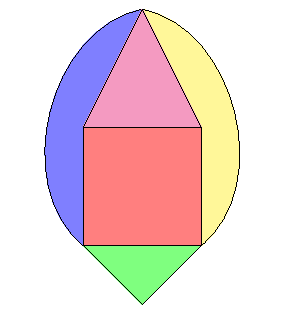
\includegraphics[width=.6\textwidth]{cauchy_images/pyramid-euler-2.pdf}%%loss of convexity
                \caption{can be flattened out}
                \label{fig:my_label}
            \end{figure}
        }
        \only<6-11>{
            \begin{figure}
                \centering
                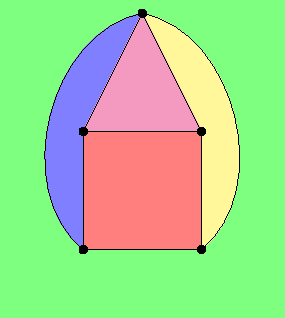
\includegraphics[width=.6\textwidth]{cauchy_images/pyramid-euler-3-pts0.pdf}%%loss of convexity
                \caption{Topological graph}
                \label{fig:my_label}
            \end{figure}
        }
        \only<12>{
            \begin{figure}
                \centering
                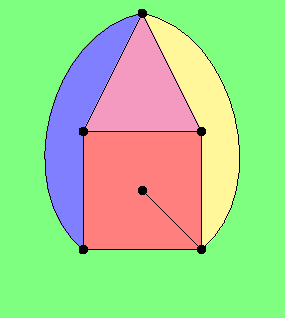
\includegraphics[width=.6\textwidth]{cauchy_images/pyramid-euler-3-pts1.pdf}%%loss of convexity
                \caption{Topological graph}
                \label{fig:my_label}
            \end{figure}
        }
        \only<13>{
            \begin{figure}
                \centering
                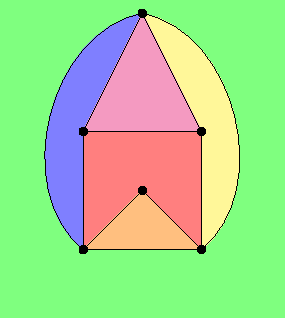
\includegraphics[width=.6\textwidth]{cauchy_images/pyramid-euler-3-pts2.pdf}%%loss of convexity
                \caption{Topological graph}
                \label{fig:my_label}
            \end{figure}
        }
        \only<14>{
            \begin{figure}
                \centering
                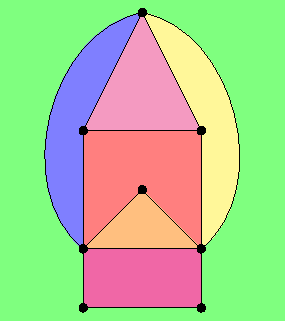
\includegraphics[width=.6\textwidth]{cauchy_images/pyramid-euler-3-pts3.pdf}%%loss of convexity
                \caption{Topological graph}
                \label{fig:my_label}
            \end{figure}
        }
        \only<15->{
            \begin{figure}
                \centering
                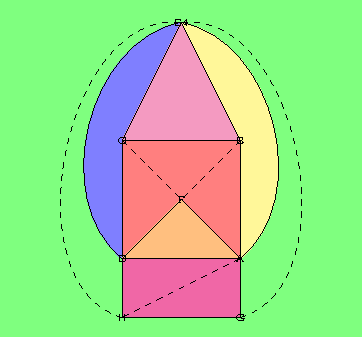
\includegraphics[width=.6\textwidth]{cauchy_images/pyramid-euler-3-pts4-triangulated.pdf}%%loss of convexity
                \caption{Topological graph}
                \label{fig:my_label}
            \end{figure}
        }
        \end{column}
    \end{columns}
    \vspace{0pt}
    \only<11->{\textbf{Euler characteristic for a topological sphere}:\\
    \textit{$V-E+F=2$}}
\end{frame}

%%%new slide%%%%
\begin{frame}{Global vs.\ Local} \label{arm lemma wrong 3}
    \center{$M$ is the number of changes.}
    \begin{columns}
        \begin{column}{.5\textwidth}
        \only<1>{
            \begin{figure}
                \centering
                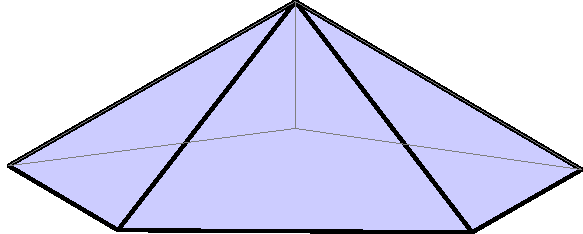
\includegraphics[width=.65\textwidth]{cauchy_images/deltahedron_top.pdf}
                % \caption{Caption}
                \label{fig:my_label}
            \end{figure}
        }
        \only<11->{
            \begin{itemize}
                \item[] \textbf{Global}
                \item<11-> Trick is to count $M$ on faces.
                \item[]<12-> Triangles: $2f_{3}$
                \item[]<13-> Squares: $4f_{4}$
                \item[]<14-> Pentagons: $4f_{5}$
                \item[]\only<11->{
                        \begin{figure}
                            \centering
                            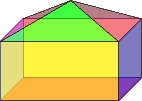
\includegraphics{cauchy_images/convex_poly.pdf}
                            \label{fig:my_label}
                        \end{figure}
                        }
                \item[]<14->\begin{block}{}
                    $2f_{3}+4f_{4}+4f_{5}+6f_{6}\dots \geq M$
                    \end{block}
            \end{itemize}
        }
        \vspace{-5pt}

        \end{column}
        
        \begin{column}{.5\textwidth}
            \only<1->{
            \begin{itemize}
                \item[] \textbf{Local $M\geq 4V$}
                \item \only<2>{$F=$ triangles+squares+pentagons+\dots} \only<3-5>{$F=f_{3}+f_{4}+f_{5}\dots$} \only<6->{$4\cdot F=4f_{3}+4f_{4}+4f_{5}\dots$}
                \item<4-> \only<4-5>{$2\cdot E= 3f_{3}+4f_{4}+5f_{5}\dots$}\only<6->{$4\cdot E= 6f_{3}+8f{4}+10f_{5}\dots$}\
                \item<5-> $V-E+F=2$%
                \item[]<7->$\Rightarrow 4V-4E+4F=8$
                \item[]<8->$\Rightarrow 4V-8=4E-4F$
                \item[]<9->$\Rightarrow 4V-8=2f_{3}+4f_{4}+6f_{5}\dots$
                \item[]
                \item[]<10->\begin{block}{}
                $M>4V-8=2f_{3}+4f_{4}+6f_{5}+8f_{6}\dots$
                \end{block}
            \end{itemize}
            }
        \end{column}
    \end{columns}
\end{frame}

%%%new slide
\begin{frame}{Global vs.~Local: The finale} \label{arm lemma wrong 4}
    \begin{columns}
        \begin{column}{.5\textwidth}
        \only<1->{
            \begin{itemize}
                \item[] \textbf{Global}
                \item[]\begin{block}{}$2f_{3}+4f_{4}+4f_{5}+6f_{6}\dots \geq M$\end{block}
            \end{itemize}
        }
        \vspace{-5pt}

        \end{column}
        
        \begin{column}{.5\textwidth}
            \only<1->{
            \begin{itemize}
                \item[] \textbf{Local $M>4V$}
                \item[]\begin{block}{}$M>2f_{3}+4f_{4}+6f_{5}+8f_{6}\dots$ \end{block}
            \end{itemize}
            }
        \end{column}
    \end{columns}
    \vspace{35pt}
    \begin{center}
        \only<3->{Assume two different polyhedrons exist\dots}
        \only<4->{$2f_{3}+4f_{4}+4f_{5}+6f_{6}\dots \geq M >2f_{3}+4f_{4}+6f_{5}+8f_{6}\dots$}
    \end{center}
    \begin{itemize}
        \item<5-> But what if all hinge angles at $k$ vertices don't change? 
        \item[]<6-> Remove those vertices $\Rightarrow$ $V-E+F =2 +k$, which helps our case above. 
    \end{itemize}
\end{frame}

\begin{frame}{200 years of relevance}
    \only<+>{
        \vspace{25pt}
        \begin{itemize}
            \item \href{https://twitter.com/johncarlosbaez/status/1064214339886866434}{Non-convex polyhedron aren't necessarily rigid.}
            \item First example was found in 1977 (Connelly). 
            \item In 1997 it was shown that the volume is constant! (Connelly, Sabitov, and Walz)
            \item Many open questions about polyhedron remain.
        \end{itemize}
    }
    \only<+>{
        \begin{figure}
            \centering
            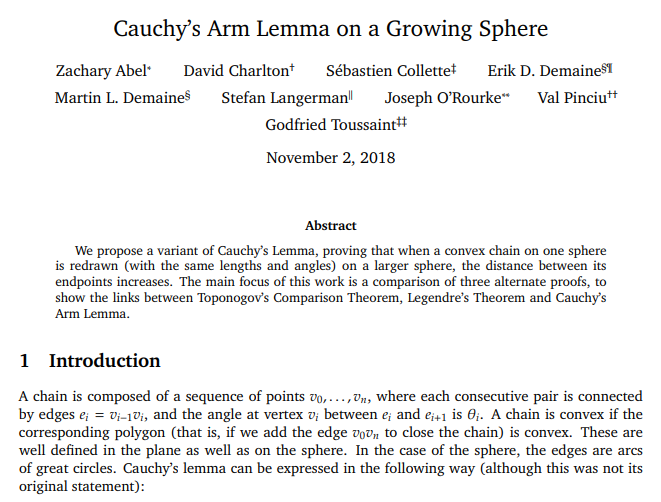
\includegraphics[width=.8\textwidth]{cauchy_images/2020-05-05_22h38_59.png}
            \label{fig:my_label}
        \end{figure}
    }
    \only<+>{
        \begin{figure}
            \centering
            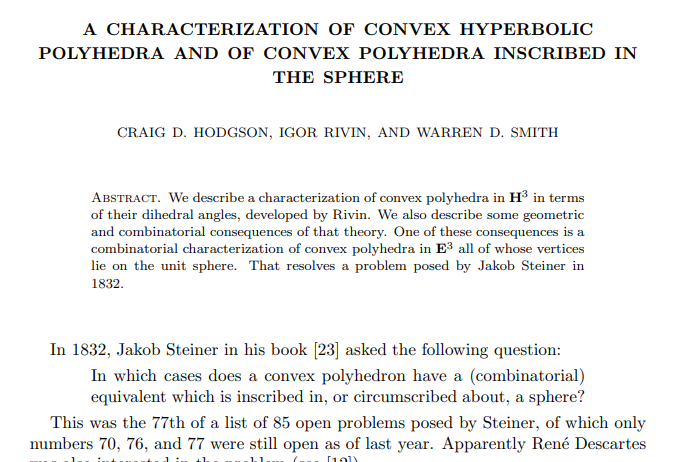
\includegraphics[width=.8\textwidth]{cauchy_images/2020-05-05_22h34_14.png}
            \label{fig:my_label}
        \end{figure}
    }
    \only<+>{
        \begin{figure}
            \centering
            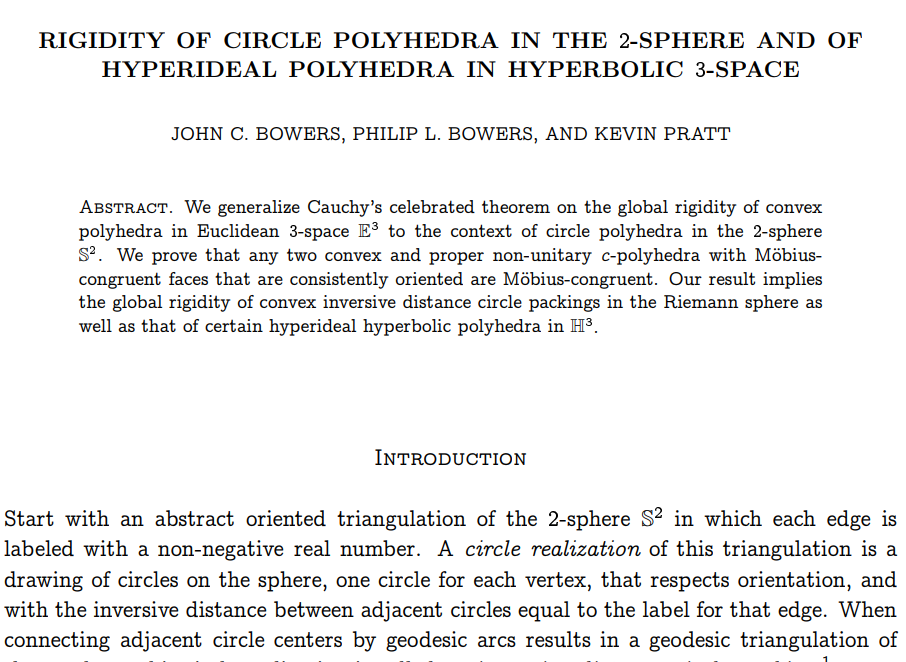
\includegraphics[width=.8\textwidth]{cauchy_images/2020-05-05_22h35_18.png}
            \label{fig:my_label}
        \end{figure}
    }
    \only<+>{
        \begin{figure}
            \centering
            
\includegraphics[width=.8\textwidth]{cauchy_images/2020-05-05_22h37_39.png}
            \label{fig:my_label}
        \end{figure}
    }
    \only<+>{
        \begin{figure}
            \centering
            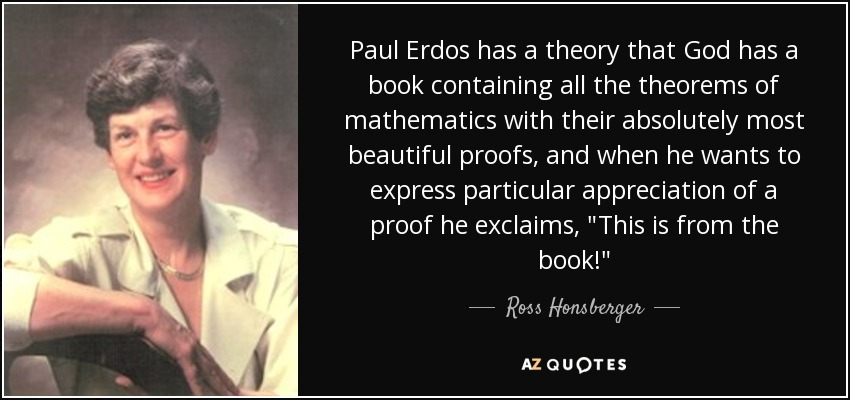
\includegraphics[width=.8\textwidth]{cauchy_images/quote-paul-erdos-has-a-theory-that-god-has-a-book-containing-all-the-theorems-of-mathematics-ross-honsberger-67-6-0601.jpg}
            \label{fig:my_label}
        \end{figure}
    }
    \only<+>{
        \begin{figure}
            \centering
            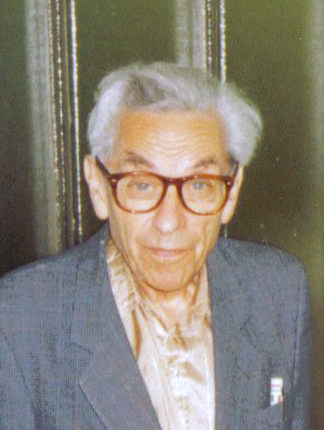
\includegraphics[width=.5\textwidth]{cauchy_images/Erdos_budapest_fall_1992_(cropped).jpg}
            \label{fig:my_label}
        \end{figure}
    }
\end{frame}

% %%%%%new slide%%%%%%%
\begin{frame}{Things people want to talk about} \label{slide-8}
    \begin{itemize} \small
        \item Machine learning and AI algorithms, e.g. how do advertisers know what to show me? How do deep fakes work? How can AI help find struggling students? How can AI help make better course materials? Monstrous moonshine?
        \item Formal methods, some of my work with the NSA
        \item Details about our 5-12 courses to those outside Teacher's College
        \item  Cauchy's thm, circle packing, Riemann's hypothesis, tiling, P!=NP(?) 
        \item Base number systems
        \item "A framework for understanding student's ways of knowing mathematics, and how it helps teaching them"
        \item Confocal microscopy in biomedical engineering or present a published paper from a math-related journal
        \item Strong differentiation in industry between engineers with strong math skills and engineers without. (Hint: more math is better).
        %%%%
    \end{itemize}
\end{frame}

%%%%%new slide%%%%%%%
\begin{frame}{Things people want to hear about} \label{slide-9}
    \begin{itemize} \small
        \only<1>{
        \item Other ideas on teaching methods from other groups.
        \item Demonstration of a math subject matter such as Geometry, Trig, Probability.
        \item How to develop better math skills in students
        \item No preference
        \item Anything!
        \item Any and everything math related! I am in Elem Math Methods, but interested in all aspects of math. 
        \item All of the things you described would be great.
        \item How folks are staying involved in mathematics, things that are working with your students, and good math reads (books, articles, blogs, etc.)
        \item Anything math or CI related is fine.
        \item Anything my peers would like to share 
        }
        %%%%
        \only<2->{
        \item I would like to know more about math courses of study outside the TC.
        \item Previous and ongoing research interests, WGU-related research, online math teaching strategies
        \item Math and how to support students
        \item current events, challenges, impacts, solutions, etc. 
        \item Maths
        \item Whatever topics other mathies feel like sharing
        \item CI strategies both personal and technological, AND 'fun' slightly-advanced math
        \item Current math news, neat facts, "on this day" in math history, teaching strategies, research interests; journal club - present published research from a math-related journal (not necessarily our own work) and allow discussion time
        }
    \end{itemize}
\end{frame}

%%%%%new slide%%%%%%%
\begin{frame}{} \label{slide-end}
    \center
    \Huge That is all
\end{frame}
%%%END SLIDES%%%
\end{document}
